\textbf{Software Testing }
\begin{flushleft}
Obwohl das Projekt relativ klein ist, wurde die Wichtigkeit von automatisierten Tests nicht unterschätzt.
\\
Für das Frontend wurden End-to-End Testfälle mit Cypress geschrieben.
Auf diese Weise ist es möglich in Sekundenschnelle festzustellen, ob etwas in unserer Anwendung defekt ist.

Ein Szenario, in dem dies hilfreich ist, ist, wenn eine Unterkomponente in anderen Komponenten verwendet wird.

Durch die Änderung der Unterkomponente kann sich diese in einer unerwünschten Weise verhalten.
\\
Das ist der Fall bei der Komponente AvatarImage.
Dies ist eine Funktionskomponente, die 3 Parameter erhält: Größe des Bildes, Bild-URL und Benutzername.

Zu Beginn des Projekts wurde nicht daran gedacht, die Größe des Bildes über einen Parameter dieser Funktion zu steuern. Im Laufe des Projekts wurde uns klar, dass wir die Logik in diesem Element wiederverwenden konnten.
\\
Innerhalb der Komponente wird geprüft, ob eine URL existiert, und wenn ja, wird das mit dem Link verbundene Bild gezeichnet. Falls es keine URL  angegeben wurde, werden die ersten beiden Buchstaben des Benutzernamens verwendet, um ein Standardsymbol zu erzeugen.

In der aktuellen Version des Codes wird diese Komponente in vier anderen Komponenten wieder verwendet.
Wenn das Projekt weiter wachsen würde, würde auch die Möglichkeit von Fehlern im Code zunehmen. Fehler zu finden, wäre in dem Fall aufwändiger.

Ohne automatisierte Tests, ist manuelles Testing nötig.
\\
Im Anhang 2 befindet sich ein Code-Auszug eines Testfälles End-to-End. 
\end{flushleft}


%%POSIBLEMENTE ESTE NO ES ELMEJOR EJ PUESTO QUE NO SE ESTA PROBANDO EL TAMANIO LAS IMAGENES EN LAS PRUEBAS DE CYPRESS
%% SIN EMBARGO EL HECHO DE REUTILIZAR LOGICA DE CIERTOS ELEMENTOS ES MUY RELEVANTE Y DEBERIA SER INCLUIDA EN OTRA PARTE %DEL REPORTE
%BUSCAR OTRO EJ. DONDE EL TESTING COBRA MAS RELEVANCIA

\subsection{Die Testfälle für unser Projekt}
\paragraph{}
Nachstehend einer Überblick über die Testfälle bei Cypress.
\\
\begin{center}
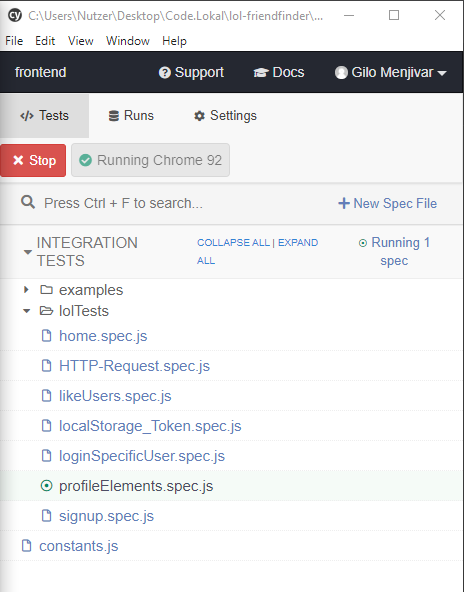
\includegraphics[scale=0.60]{Cy_Test_Cases}\label{fig:Cy_Test_Cases}\\
\textbf{Abbildung \autoref{fig:Cy_Test_Cases}:} Testfälle in Cypress
\end{center}

\begin{center}
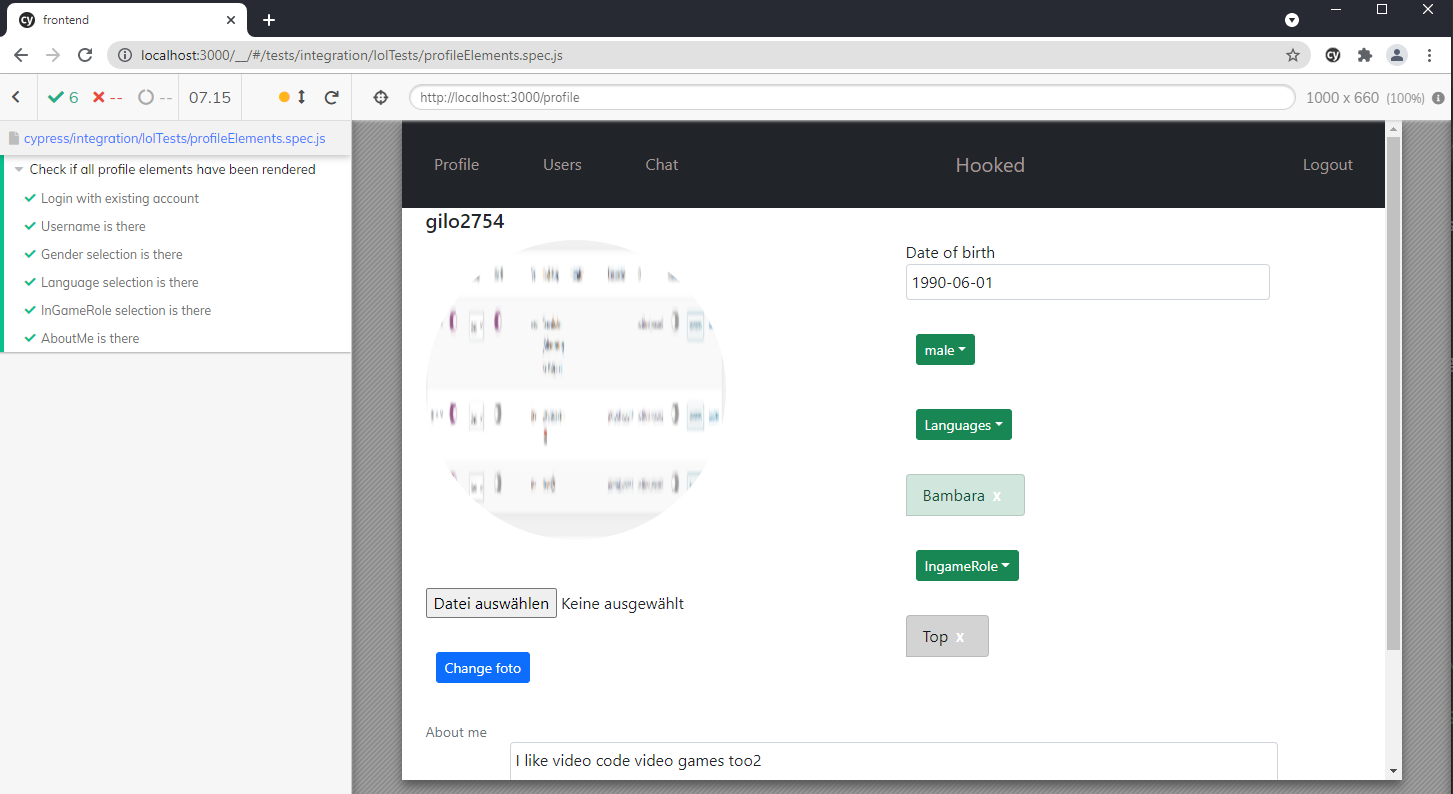
\includegraphics[scale=0.40]{Cy_Test_running}\label{fig:Cy_Test_running}
\textbf{Abbildung \autoref{fig:Cy_Test_running}:} Grafische Darstellung der verschiedenen Tests in Cypress
\end{center}

\newpage
\textbf{home.spec.js}\\
Prüfen Sie, ob die Startseite „Home“ gerendert wurde.
\\\\
\textbf{likeUsers.spec.js}\\
Mit diesem Testfall wird überprüft, ob nach der Vergabe von einem „Like“ oder einem „Dislike“ ein anderer Nutzer angezeigt wird.
\\\\
\textbf{Testfall localStorage Token}\\
Hier wird der Wert des JSON-Web-Tokens zu verschiedenen Zeitpunkten überprüft.
Die Erwartung ist, dass das Token null ist, wenn der Benutzer nicht angemeldet ist.
Dieses Token wird in localStorage gespeichert.
Es besteht auch die Möglichkeit, dass das Token abgelaufen ist, wodurch alle Abfragen an den Server, die eine Authentifizierung erfordern, unmöglich werden.
\\\\
\textbf{profileElements.spec.js}\\
Der Testfall prüft, ob die Elemente und Komponenten der Komponente Profil gerendert wurden und sichtbar sind. Diese Elemente sind userName, Gender und AboutMe. Die Komponenten sind Language und InGameRole.
Außerdem wird überprüft, ob Komponenten, ein Element „Dropdown“ enthalten, eine Mindestanzahl von Elementen enthalten, die angezeigt werden müssen. 
\\\\
\textbf{signUp.spec.js}\\
Dieser Testfall erstellt einen neuen Benutzer mit einer zufälligen E-Mail und einem zufälligen Benutzernamen.  \\
\\
\textbf{Commands bei Cypress}\\
\begin{flushleft}
In den Testfällen gibt es Aktionen, die sich immer wieder wiederholen, zum Beispiel die Anmeldung eines Nutzers.
\\
Zu diesem Zweck wurde in Cypress ein wiederverwendbarer Befehl definiert.
\\
Diese setzen sich aus nativen Cypress-Befehlen zusammen. Es handelt sich praktisch um benutzerdefinierte Funktionen, die häufig bei Tests verwendet werden.

Ein Beispiel ist im Anhang 3 zu finden.
\end{flushleft}

%Ergebnise der ganzen Testlauf